\section{Background Modeling}
\label{bkg_model}
Given highly dominant nature of background processes, it is important to properly model the background shape as that is the biggest contributor for any physical quantity of interest that we are to compute. In general, our background can be described by means of falling exponential with some polynomial contribution.

The background is mainly composed by Drell--Yan and top pair production ($t\bar{t}$). MC samples for such processes are available at NLO (2j) and NNLO (incl), but they are not suited to be used for background modeling directly because they have little statistical power with respect to the data in the region of interests as well as large statistical uncertainties due to extra terms in QCD or EW expansions (high $\pt$), as well as resummation (low $\pt$), pdf and scale uncertainties, and unknown modeling of the long range correlation uncertainties. Therefore, we choose to treat the modeling of background using smooth functional forms.

% Models: Physcs Motivated Models and Polynomial-like Families
For the purpose of modeling, we identify two classes of models that we consider: physics motivated models and general purpose series able to describle any smoothly falling functional forms (polynomials, sum of exponentials). The first class contains several pdfs whose functional forms are driven by the knowledge of background processes contributing the most (Drell-Yan, ttbar). The functions considered are summarized in eqs~\ref{eq:ExpPol2}-\ref{eq:BWZGamma}.
\begin{align}
        \label{eq:ExpPol2}
        \text{ExpPolynomial:}& {B(x)} = {e^{a_{1}x + a_{2}x^2}} \\
        \label{eq:BWZ}
        \text{BWZ:}& {B(x)} = {\frac{e^{ax}\sigma_{z}}{(x-\mu_{z})^2 + (\frac{\sigma_{z}}{2})^2}} \\
        \label{eq:BWZRedux}
        \text{BWZRedux:}& {B(x)} = {\frac{e^{a_{2}x + a_{3}x^2}}{(x-\mu_{z})^{a_{1}} + (\frac{2.5}{2})^{a_{1}}}} \\
        \label{eq:BWZGamma}
        \text{BWZGamma:}& {B(x)} = {f\frac{e^{ax}\sigma_{z}}{(x-\mu_{z})^2 + (\frac{\sigma_{z}}{2})^2} + (1-f)\frac{e^{ax}}{x^2}}
\end{align}

These shapes have been derived and validated fitting the FEWZ (NNLO QCD) generated mass shapes (consult the \cite{CMS-HIG-AN}) and the fitted values for the parameters have been used as initial guesses for the modeling procedure. The second class of functions we consider comes from general families which are, in principle, capable of describing any functional form by incorporating more and more terms. We consider several families, polynomials in the Bernstein basis, power law, and sum of exponentials, summurized in eqs~\ref{eq:Bernstein}-\ref{eq:Laurent}.
\begin{align}
        \label{eq:Bernstein}
        \text{Bernsteins:}& {B(x)} = {\sum_{i=0}^{n} \alpha_i[\binom{n}{i}x^{i}(1-x)^{n-i}]} \\
        \label{eq:SumExponentials}
        \text{SumExponentials:}& {B(x)} = {\sum_{i=1}^{n} \beta_{i}e^{\alpha_{i}x}}\\
        \label{eq:SumPowers}
        \text{SumPowers:}& {B(x)} = {\sum_{i=1}^{n} \beta_{i}x^{\alpha_{i}}}\\
        \label{eq:Laurent}
        \text{LaurentSeries:}& {B(x)} = {\sum_{i} \alpha_{i}x^{i}}
\end{align}

% Figure~\ref{bkgmodel:exampleModels} shows several examples of background only fits to the data for various hypothetical functional forms. From left to right, we have functions being fit for the mass ranges [110, 160] \gev, [110, 200] \gev and [110, 250] \gev. For the full list of those, please refer to Appendix \textbf{FIXME}.
% \begin{figure}[hbp]
%      \centering
%      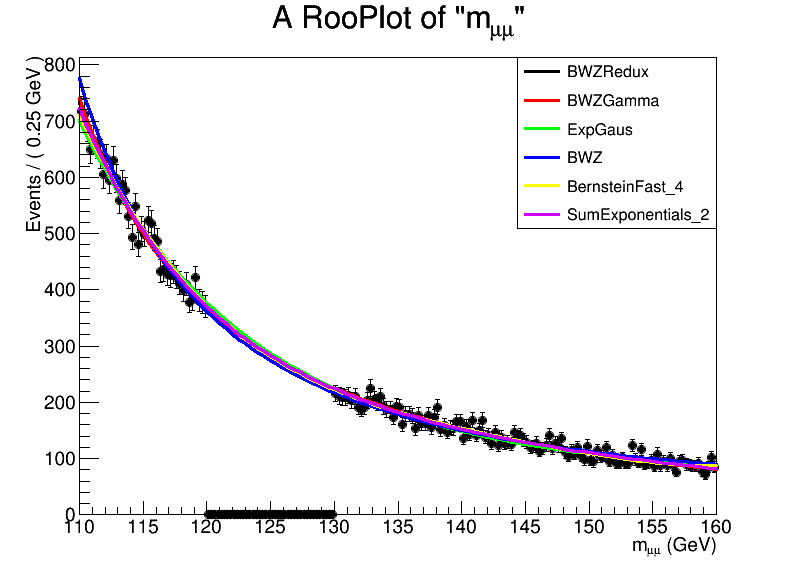
\includegraphics[width=0.3\textwidth]{figures/background_model/baseline_p25GeV_110to160/backgroundFits__01JetsTightBB__bkgModels.png}
%      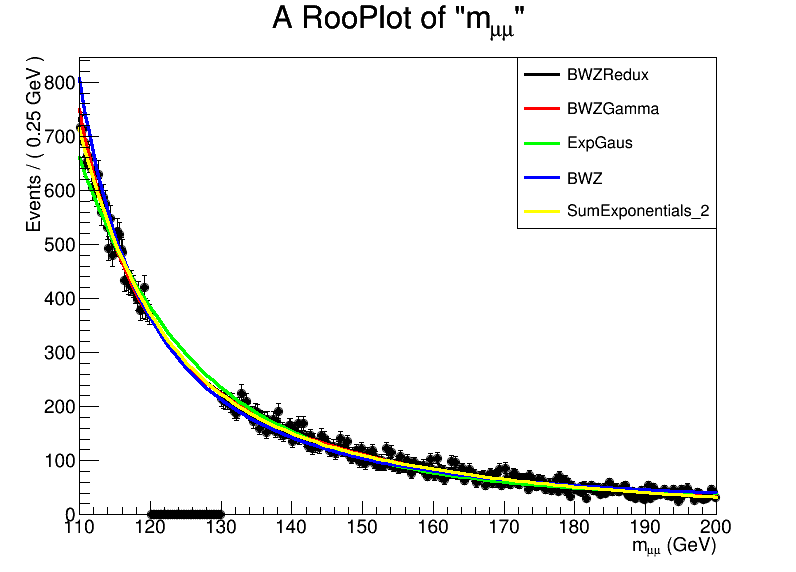
\includegraphics[width=0.3\textwidth]{figures/background_model/baseline_p25GeV_110to200/backgroundFits__01JetsTightBB__bkgModels.png}
%      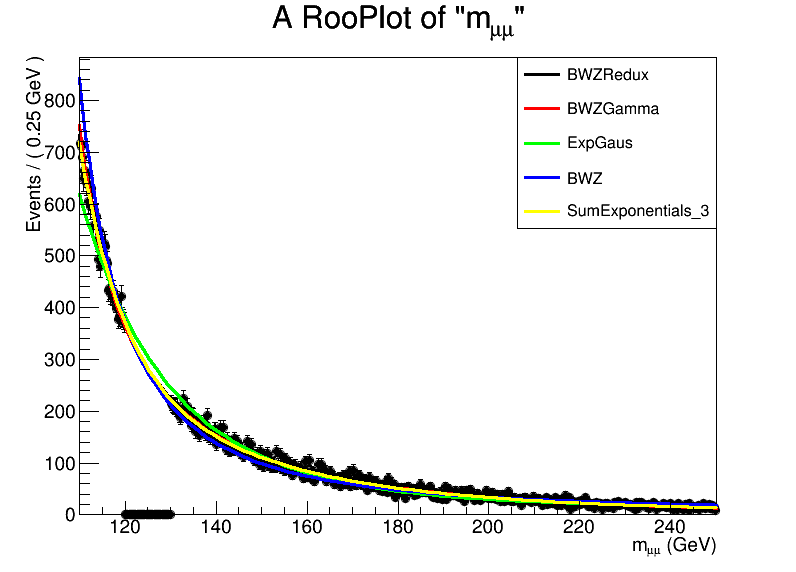
\includegraphics[width=0.3\textwidth]{figures/background_model/baseline_p25GeV_110to250/backgroundFits__01JetsTightBB__bkgModels.png}
%      \caption{}
%      \label{bkgmodel:exampleModels}
%  \end{figure}

 The background modeling procedure involves the construction of an envelope (RooMultiPdf) of pdfs that can either be used individually or altogether (discrete profile method \cite{CMS-PAS-HIG-13-001}) for the purpose of fitting the signal strength or setting the upper limit. For the physics motivated functions, we simply perform the binned maximum likelihood fit and insert that model into the envelope. Nevertheless, the discrite profile method allows to naturally take into account the number of free parameters in the fit, the computational time it takes scales linearly with the product $n_\textup{cat}\times n_\textup{family}$, since it performs one fit for all possible combination of choices of functional forms in all categories. In order to minimize the time it takes to perform the regression, the number of families in the envelope, an order for a family gets choosen using the F-Test (Fisher Test) method at 95\% Confidence Level. The actual algorithm of the order selection for a particular family follows:
\begin{itemize}
    \item For a given category and for a particular family
    \item $H_0$ hypothesis: order $n$ is the true order. To reject this hypothesis, we have to be at least 95\% confident rejecting it, in other words: $p-\text{value}(\chi^2, ndf) < 5\%$
    \item Perform the background only fit for orders $n$ and $n+1$ to the data
    \item Compute $\chi^2_{n}$ and $\chi^2_{n+1}$ respectively. $\chi^2 = -2\log\mathcal{L}$
    \item Compute the difference in the number of degrees of freedom: $\Delta NDF = NDF_{n+1} - NDF_{n}$
    \item $\chi^2 = \chi^2_{n+1} - \chi^2_{n} = -2\Delta\log\mathcal{L}$. Note, that $\chi^2_1 + \chi^2_2$ is also distributed as a $\chi^2$, but with $NDF = NDF_1 + NDF_2$.
    % \item use $\chi^2_ = 2 \Delta \log\mathcal{L}$, as for the asymptotic approximation of the Likelihood function.
    % \item compute the difference in number of degrees of freedom $\text{n.d.f.} = \text{NDF}_{n+1} - \text{NDF}_{n}$
    % \item the $\chi^2$ variable is distributed as a $\chi^2$-distribution with $\text{n.d.f.}$ degrees of freedom,
    \item Compute the $\chi^2$ p-value
    \item For p-value less than 5\%, we are rejecting n and move on to test n+1
    \item For p-value greater than 5\%, we stop and select order $n$ for this category, for this functional family.
\end{itemize}

Figures~\ref{fig:higgs_bmodel_bdtc1c3}-~\ref{fig:higgs_bmodel_bdtc10c12} shows the dimuon mass distributions together with the background envelope of analytic functions fitted to the data. The binned maximum likelihood fit is performed. The order of a family is chosen using the F-Test procedure described just above and varies depending on the category.
\begin{figure}[hbp]
  \centering
  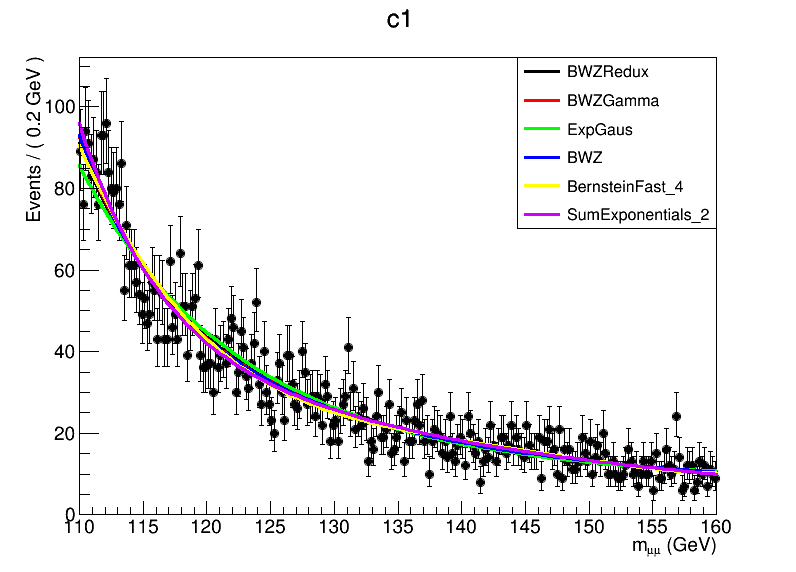
\includegraphics[width=0.65\linewidth]{figures/ch_higgs/backgroundmodel/uf_bdt/backgroundFits__c1__bkgModels.png}\\
  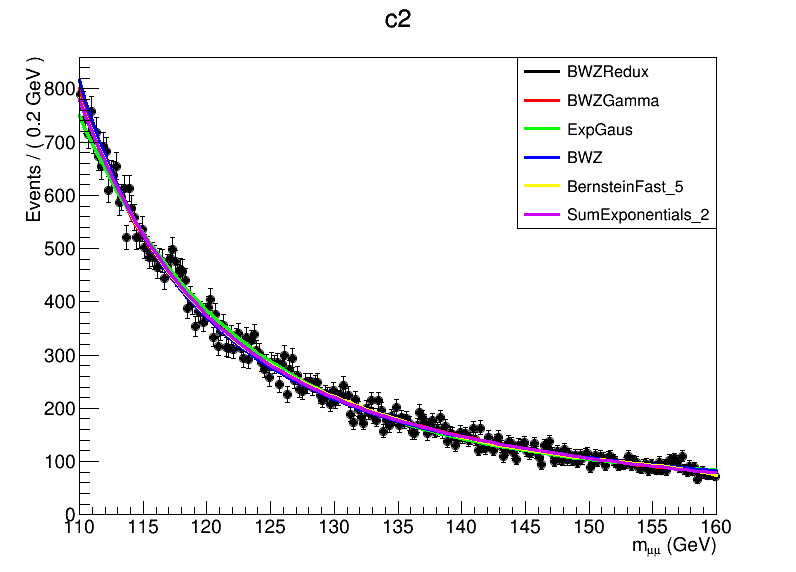
\includegraphics[width=0.65\linewidth]{figures/ch_higgs/backgroundmodel/uf_bdt/backgroundFits__c2__bkgModels.png}\\
  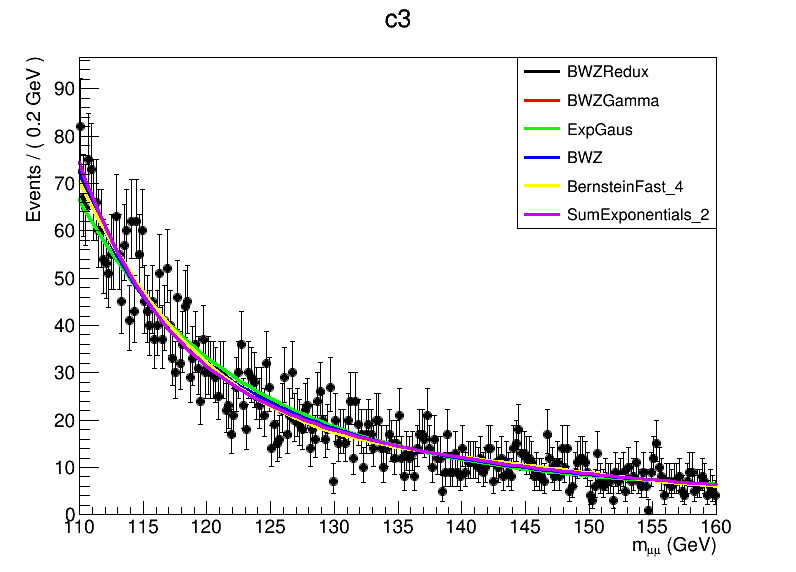
\includegraphics[width=0.65\linewidth]{figures/ch_higgs/backgroundmodel/uf_bdt/backgroundFits__c3__bkgModels.png}
  \caption{Background Modeling envelope of analytic functions fitted to the data (c1 - c3)}
  \label{fig:higgs_bmodel_bdtc1c3}
\end{figure}
\begin{figure}[hbp]
  \centering
  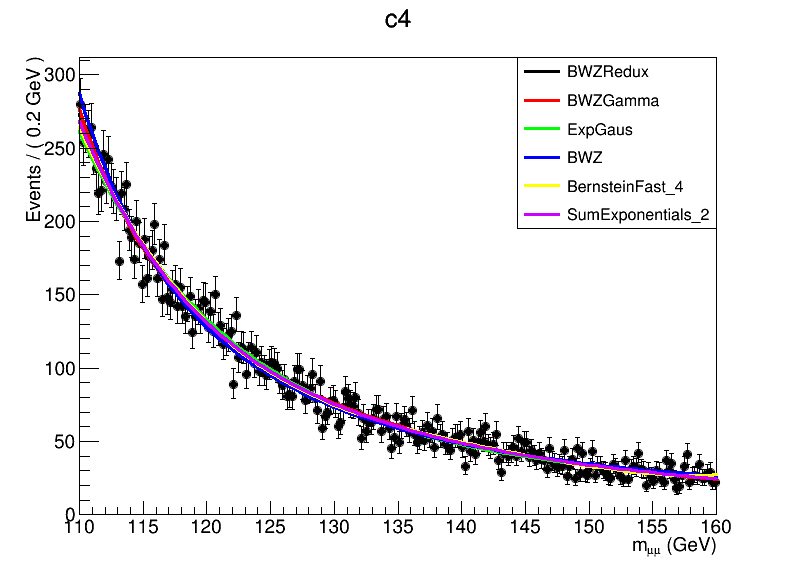
\includegraphics[width=0.65\linewidth]{figures/ch_higgs/backgroundmodel/uf_bdt/backgroundFits__c4__bkgModels.png}\\
  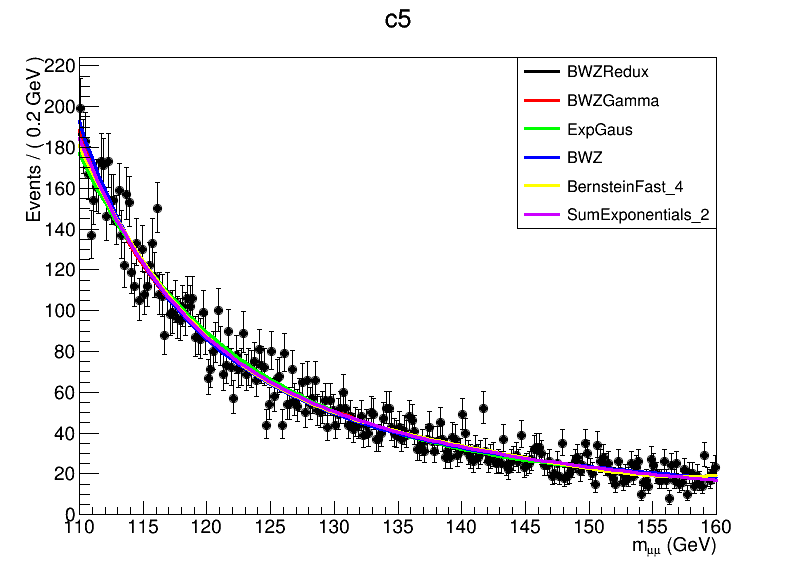
\includegraphics[width=0.65\linewidth]{figures/ch_higgs/backgroundmodel/uf_bdt/backgroundFits__c5__bkgModels.png}\\
  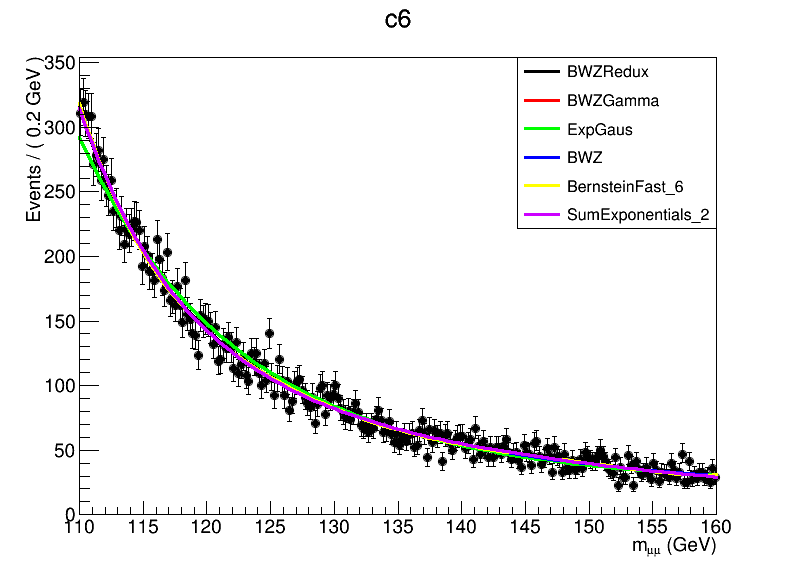
\includegraphics[width=0.65\linewidth]{figures/ch_higgs/backgroundmodel/uf_bdt/backgroundFits__c6__bkgModels.png}
  \caption{Background Modeling envelope of analytic functions fitted to the data (c4 - c6)}
  \label{fig:higgs_bmodel_bdtc4c6}
\end{figure}
\begin{figure}[hbp]
  \centering
  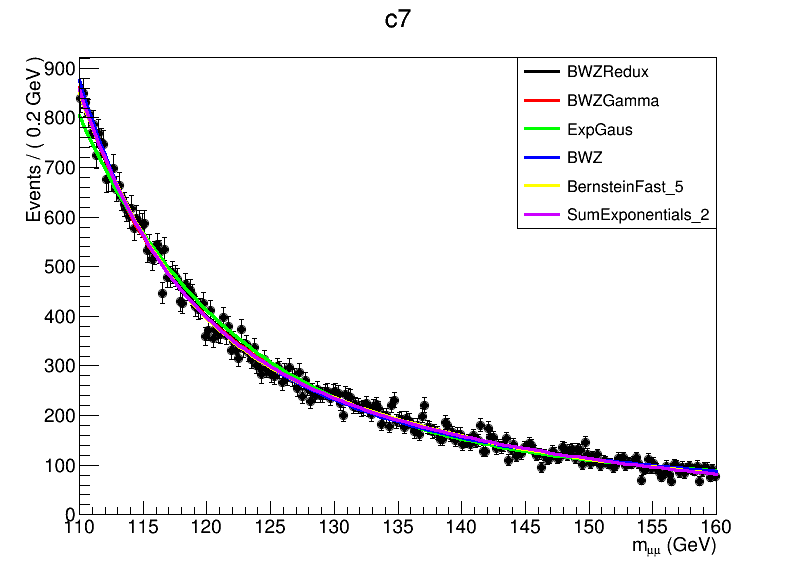
\includegraphics[width=0.65\linewidth]{figures/ch_higgs/backgroundmodel/uf_bdt/backgroundFits__c7__bkgModels.png}\\
  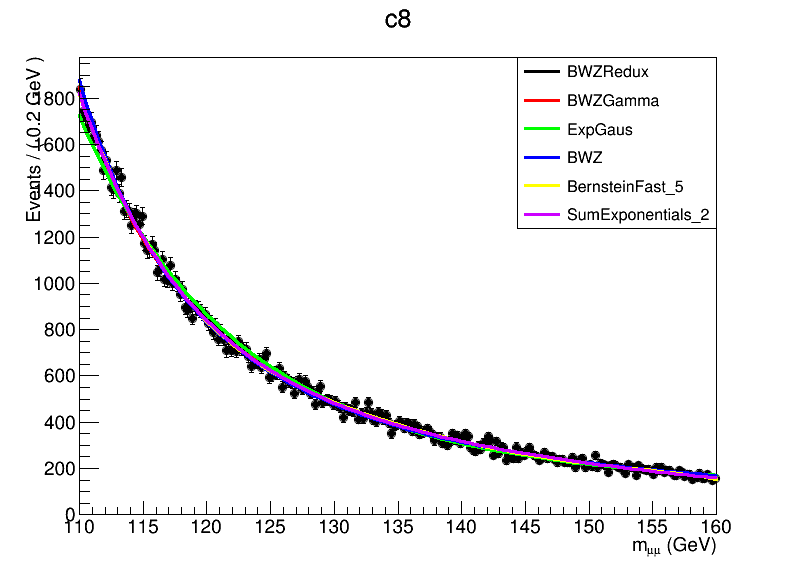
\includegraphics[width=0.65\linewidth]{figures/ch_higgs/backgroundmodel/uf_bdt/backgroundFits__c8__bkgModels.png}\\
  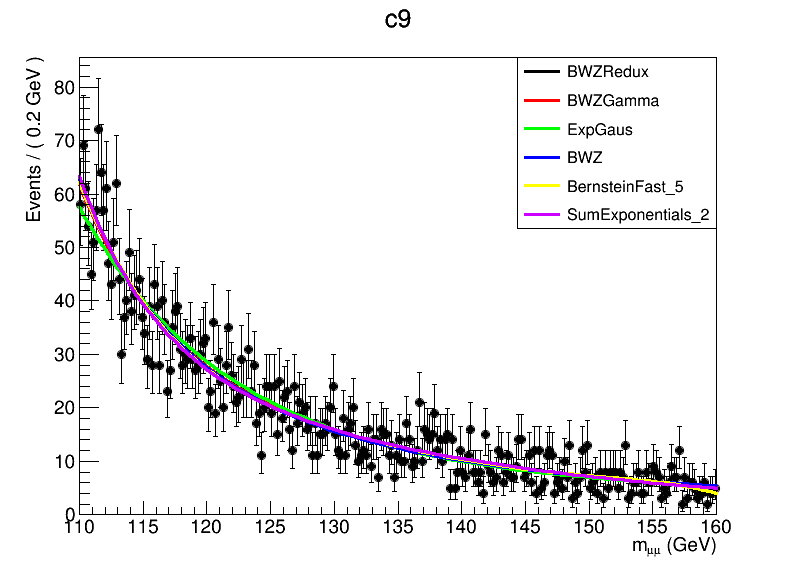
\includegraphics[width=0.65\linewidth]{figures/ch_higgs/backgroundmodel/uf_bdt/backgroundFits__c9__bkgModels.png}
  \caption{Background Modeling envelope of analytic functions fitted to the data (c7 - c9)}
  \label{fig:higgs_bmodel_bdtc7c9}
\end{figure}
\begin{figure}[hbp]
  \centering
  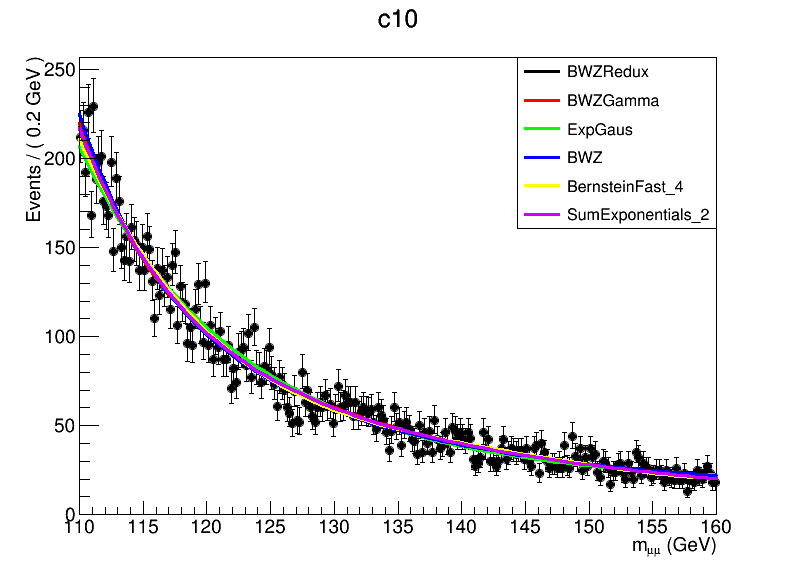
\includegraphics[width=0.65\linewidth]{figures/ch_higgs/backgroundmodel/uf_bdt/backgroundFits__c10__bkgModels.png}\\
  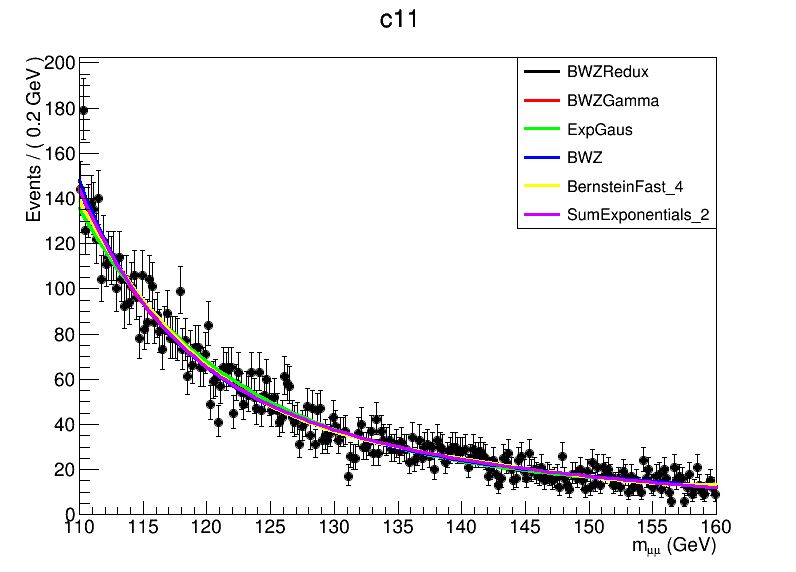
\includegraphics[width=0.65\linewidth]{figures/ch_higgs/backgroundmodel/uf_bdt/backgroundFits__c11__bkgModels.png}\\
  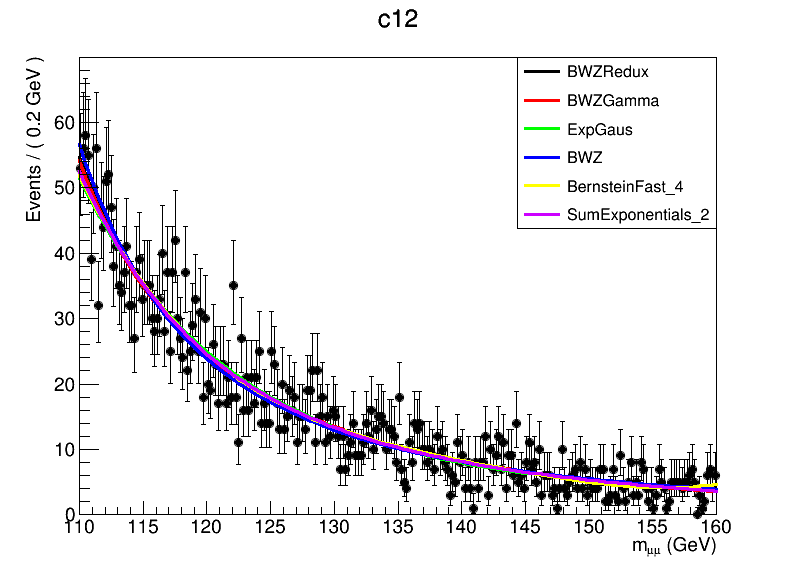
\includegraphics[width=0.65\linewidth]{figures/ch_higgs/backgroundmodel/uf_bdt/backgroundFits__c12__bkgModels.png}
  \caption{}
  \label{fig:higgs_bmodel_bdtc10c12}
\end{figure}